% Tento soubor nahraďte vlastním souborem s přílohami (nadpisy níže jsou pouze pro příklad)
% This file should be replaced with your file with an appendices (headings below are examples only)

% Umístění obsahu paměťového média do příloh je vhodné konzultovat s vedoucím
% Placing of table of contents of the memory media here should be consulted with a supervisor
\chapter{Obsah přiloženého paměťového média}
\begin{itemize}
\item \texttt{/processing\_steps}: adresář obsahuje podadresáře \texttt{/7}\,(serverová část) a \texttt{/8a}\,(klientská část).
\item \texttt{/collPart001}: obsahuje soubor \texttt{example.mg4j} a podadresář \texttt{/final} s indexy. 
\item \texttt{/thesis}: zdrojový kód technické zprávy.
\item \texttt{projekt.pdf}: technická zpráva ve formátu PDF, verze pro WIS.
\item \texttt{projekt\_tisk.pdf}: technická zpráva ve formátu PDF, verze pro tisk.
\item \texttt{plakat.pdf}: plakát.
\item \texttt{query.pdf}: dokumentace k balíku \textbf{query}.
\end{itemize}

\chapter{Manuál}

Příloha popisuje návod na použití serverové a klientské aplikace.

\section{Zprovoznění serverové aplikace}
Pro kompilaci se používá  \emph{Apache Maven 3.3}\footnote{\href{https://maven.apache.org/download.cgi}{https://maven.apache.org/download.cgi}}. Zdrojové soubory programu určeného pro sémantické indexování se nacházejí v adresáři:
\begin{itemize}
\item \texttt{./processing\_steps/7/corpproc}
\end{itemize}
Kompilace se provádí příkazem:
\begin{itemize}
\item \texttt{mvn package}
\end{itemize}
Pokud aktuální prostředí používá \emph{Java 7}, je potřeba nainstalovat a přepnout na \emph{Java 8}:
\begin{itemize}
\item \texttt{export JAVA\_HOME=/usr/lib/jvm/java-8-oracle}
\end{itemize}
Pro indexaci je zapotřebí mít adresář s uloženými soubory ve formátu mg4j:
\begin{itemize}
\item \texttt{mkdir cesta/collPart001; cp *.mg4j cesta/collPart001}
\end{itemize}
Dále je zapotřebí provést indexování:
\begin{itemize}
\item \texttt{java -jar target/corpproc-1.0-SNAPSHOT-jar-with-dependencies.jar \hfill \break
-c src/main/resources/config.yaml index cesta/collPart001 \hfill \break cesta/collPart001/final}
\end{itemize}
Po provedení indexování lze spustit serverovou část:
\begin{itemize}
\item \texttt{java -jar target/corpproc-1.0-SNAPSHOT-jar-with-dependencies.jar \hfill \break
-c src/main/resources/config.yaml serve cesta/collPart001/final}
\end{itemize}

\section{Zprovoznění klientské aplikace}
Pro kompilaci se používá \emph{Apache Maven 3.3} a pro spouštění \emph{Java 8}.
Zdrojové soubory programu jsou v adresáři:
\begin{itemize}
\item \texttt{./processing\_steps/8a/mg4jquery}
\end{itemize}
Kompilace se provádí příkazem:
\begin{itemize}
\item \texttt{mvn compile assembly:single}
\end{itemize}
% Aplikace pracuje s parametry:
% \begin{itemize}
% \item \texttt{-s|-\,-snippets}: určuje počet očekávaných snippetů\,(0 znamená vrátit vše)
% \item \texttt{-q|-\,-query}: určuje dotaz v jazyce MG4J-EQL
% \item \texttt{-p|-\,-config}: určuje cestu k konfiguračnímu souboru
% \item \texttt{-h|-\,-hosts}: určuje cestu k souboru se servery ve formátu \texttt{host:port}
% \item \texttt{-d|-\,-document}: určuje identifikátor dokumentu
% \item \texttt{-r|-\,-readTimeout}: určuje dobu očekávaní odpovědi
% \item \texttt{-t|-\,-thread}: určuje identifikátor kolekce
% \item \texttt{-k|-\,-keeper}: určuje adresu serveru obsahujícího dokument
% \item \texttt{-g|-\,-get}: přepínač způsobí vrácení jednoho dokumentu určeného parametry \texttt{-d}, \texttt{-k}, \texttt{-t}
% \item \texttt{-e|-\,-err}: přepínač způsobí výpis chybových hlášek
% \item \texttt{-n|-\,-next}: přepínač způsobí dotazu na další dávku snippetů 
% \end{itemize}
Dotazovaní na množství snippetů se spouští příkazem:
\begin{itemize}
\item \texttt{java -jar target/mg4jquery-0.0.1-SNAPSHOT-jar-with-dependencies.jar -s 15 -q  "nertag:person"~-h cesta/servers.txt -p src/resources/config.xml}
\end{itemize}
Dotazování na dokument se spouští příkazem:
\begin{itemize}
\item \texttt{java -jar target/mg4jquery-0.0.1-SNAPSHOT-jar-with-dependencies.jar \hfill\break
-p src/resources/config.xml -g -k 127.0.0.1:12000 -d 7 -t 0 \hfill\break -h cesta/servers.txt}
\end{itemize}
Získaní další dávky dat, určené parametrem \texttt{-s}, lze provést přidáním přepínače \texttt{-n}:
\begin{itemize}
\item \texttt{java -jar target/mg4jquery-0.0.1-SNAPSHOT-jar-with-dependencies.jar -s 15 -q  "nertag:person"~-h cesta/servers.txt -p src/resources/config.xml -n}
\end{itemize}

%\chapter{Konfigurační soubor}

%\chapter{RelaxNG Schéma konfiguračního souboru} % Scheme of RelaxNG configuration file

%\chapter{Plakat} % poster


%%%%%%%%%%%%%%%%%%%%%%%%%%%%%%%%%%%%%%%%%%%%%%%%%%%%%%%%%%%%%%%%%%%%%%%%%%%%%%%%

% \chapter{Výsledky testování}
% \section{Naměřené hodnoty}
% \label{recordedValues}
% \begin{table}
% \begin{tabular}{|c|c|c|c|c|c|}
% \hline
% \textbf{Kolekce} & \textbf{Doba\,(sec.)} & \textbf{Očekávané snippety} & \textbf{\textnumero snippetů} & \textbf{\textnumero šablon} & \textbf{Dokumenty} \\
% \hline
% \emph{collPart001} & 3.950 & 100 & 105 & 106 & 89 \\
% \hline
% \emph{collPart001} & 3.950 & 100 & 105 & 106 & 89 \\
% \hline
% \emph{collPart001} & 4.347 & 150 & 150 & 152 & 129 \\
% \hline
% \emph{collPart001} & 5.309 & 200 & 212 & 214 & 179 \\
% \hline
% \emph{collPart001} & 6.297 & 250 & 252 & 254 & 209 \\
% \hline
% \emph{collPart001} & 7.165 & 300 & 306 & 308 & 248 \\
% \hline
% \emph{collPart001} & 8.126 & 500 & 332 & 334 & 264 \\
% \hline
% \emph{collPart001} & 7.98 & all & 332 & 334 & 264 \\
% \hline
% %%%%%%%%%%%%%%%%%%%%%%%%%%%%%%%%%%%%%%%%%%%%%%%
% \emph{collPart002} & 3.411 & 100 & 107 & 109 & 80 \\
% \hline
% \emph{collPart002} & 4.455 & 150 & 164 & 161 & 120 \\
% \hline
% \emph{collPart002} & 5.143 & 200 & 205 & 210 & 160 \\
% \hline
% \emph{collPart002} & 5.83 & 250 & 254 & 259 & 200 \\
% \hline
% \emph{collPart002} & 7.042 & 300 & 308 & 313 & 250 \\
% \hline
% \emph{collPart002} & 12.263 & 500 & 507 & 515 & 408 \\
% \hline
% \emph{collPart002} & 17.172 & 1500 & 656 & 667 & 524 \\
% \hline
% \emph{collPart002} & 17.111 & all & 656 & 667 & 524 \\
% \hline
% %%%%%%%%%%%%%%%%%%%%%%%%%%%%%%%%%%%%%%%%%%%%%%%%%%%%%
% \emph{collPart003} & 3.117 & 100 & 106 & 111 & 90\\
% \hline
% \emph{collPart003} & 4.468 & 150 & 157 & 160 & 130\\
% \hline
% \emph{collPart003} & 5.832 & 200 & 208 & 212 & 170\\
% \hline
% \emph{collPart003} & 6.940 & 250 & 258 & 262 & 210\\
% \hline
% \emph{collPart003} & 7.336 & 300 & 304 & 308 & 249\\
% \hline
% \emph{collPart003} & 11.227 & 500 & 501 & 513 & 418 \\
% \hline
% \emph{collPart003} & 16.171 & 1500 & 856 & 881 & 712 \\
% \hline
% \emph{collPart003} & 21.763 & all & 856 & 881 & 712 \\
% \hline

% \end{tabular}
% \label{influencedStats}
% \caption{Statistiky při dotazu \emph{influenced}}
% \end{table}

% \begin{table}
% \begin{tabular}{|c|c|c|c|c|c|}
% \hline
% \textbf{Kolekce} & \textbf{Doba\,(sec.)} & \textbf{Očekávané snippety} & \textbf{\textnumero snippetů} & \textbf{\textnumero šablon} & \textbf{Dokumenty} \\
% \hline
% \emph{collPart001} & 1.110 & 100 & 168 & 201 & 20 \\
% \hline
% \emph{collPart001} & 2.704 & 500 & 506 & 599 & 135\\
% \hline
% \emph{collPart001} & 7.085 & 1500 & 2048 & 2048 & 472 \\
% \hline
% \emph{collPart001} & 10.611 & 5000 & 5257 & 6423 & 1212 \\
% \hline
% \emph{collPart001} & 22.639 & 10000 & 14712 & 12264 & 2770 \\
% \hline
% \emph{collPart001} &  97.409 & 50000 & 62850 & 51608 & 11930 \\
% \hline
% \emph{collPart001} &  223.234 & all & 66054 & 80354 & 15010 \\
% \hline
% %%%%%%%%%%%%%%%%%%%%%%%%%%%%%%%%%%%%%%%%%%%%%%%%%%%
% \emph{collPart002} & 1.375 & 100 & 112 & 142 & 38 \\
% \hline
% \emph{collPart002} & 3.399 & 500 & 525 & 757 & 143 \\
% \hline
% \emph{collPart002} & 7.305 & 1500 & 1572 & 2157 & 382 \\
% \hline
% \emph{collPart002} & 11.080 & 5000 & 5264 & 6787 & 1212 \\
% \hline
% \emph{collPart002} & 21.409 & 10000 & 11960 & 14810 & 2779 \\
% \hline
% \emph{collPart002} & 97.962 & 50000 & 51681 & 63400 & 11951 \\
% \hline
% \emph{collPart002} & 359.595 & all & 130786 & 160612 & 30078\\
% \hline
% %%%%%%%%%%%%%%%%%%%%%%%%%%%%%%%%%%%%%%%%%%%%%%%%%%%%
% \emph{collPart003} & 1.373 & 100 & 133 & 166 & 45 \\
% \hline
% \emph{collPart003} & 2.241 & 500 & 503 & 600 & 150 \\
% \hline
% \emph{collPart003} & 8.080 & 1500 & 2466 & 3290 & 462 \\
% \hline
% \emph{collPart003} & 17.201 & 5000 & 5226 & 6760 & 1184 \\
% \hline
% \emph{collPart003} & 31.037 & 10000 & 11380 & 14059 & 2730\\
% \hline
% \emph{collPart003} & 60.582 & 50000 & 52677 & 67095 & 11958\\
% \hline
% \emph{collPart003} & 397.242 & all & 161494 & 201415 & 37946\\
% \hline
% \end{tabular}
% \label{nertagdateStats}
% \caption{Statistiky při dotazu \emph{nertag:date}}
% \end{table}


% \begin{table}
% \begin{tabular}{|c|c|c|c|c|c|}
% \hline
% \textbf{Kolekce} & \textbf{Doba\,(sec.)} & \textbf{Očekávané snippety} & \textbf{\textnumero snippetů} & \textbf{\textnumero šablon} & \textbf{Dokumenty} \\
% \hline
% \emph{collPart001} & 1.944 & 100 & 110 & 110 & 20 \\
% \hline
% \emph{collPart001} & 5.409 & 500 & 502 & 502 & 193\\
% \hline
% \emph{collPart001} & 14.820 & 1500 & 1777 & 1777 & 568 \\
% \hline
% \emph{collPart001} & 25.099 & 5000 & 5155 & 5155 & 1991 \\
% \hline
% \emph{collPart001} & 53.769 & 10000 & 10912 & 10912 & 3798 \\
% \hline
% \emph{collPart001} &  125.272 & 50000 & 24840 & 24840 & 8904 \\
% \hline
% \emph{collPart001} &  217.301 & all & 24840 & 24840 & 8904 \\
% \hline
% %%%%%%%%%%%%%%%%%%%%%%%%%%%%%%%%%%%%%%%%%%%%%%%%%%%%%%%5
% \emph{collPart002} & 1.959 & 100 & 135 & 135 & 38 \\
% \hline
% \emph{collPart002} & 4.937 & 500 & 517 & 517 & 163 \\
% \hline
% \emph{collPart002} & 12.688 & 1500 & 1722 & 1722 & 568 \\
% \hline
% \emph{collPart002} & 26.670 & 5000 & 5264 & 6787 & 1891 \\
% \hline
% \emph{collPart002} & 52.096 & 10000 & 10302 & 10302 & 3769 \\
% \hline
% \emph{collPart002} & 242.854 & 50000 & 46789 & 46789 & 17662 \\
% \hline
% \emph{collPart002} & 359.595 & all & 46789 & 46789 & 17662\\
% \hline
% %%%%%%%%%%%%%%%%%%%%%%%%%%%%%%%%%%%%%%%%%%%%%%%%%%%%%%%%%
% \emph{collPart003} & 2.057 & 100 & 129 & 129 & 52 \\
% \hline
% \emph{collPart003} & 5.672 & 500 & 520 & 520 & 192 \\
% \hline
% \emph{collPart003} & 17.307 & 1500 & 1511 & 1511 & 461 \\
% \hline
% \emph{collPart003} & 29.827 & 5000 & 5161 & 5161 & 1979 \\
% \hline
% \emph{collPart003} & 57.079 & 10000 & 10288 & 10288 & 3788\\
% \hline
% \emph{collPart003} & 265.279 & 50000 & 51107 & 51107 & 18878\\
% \hline
% \emph{collPart003} & 529.347 & all & 60249 & 60249 & 22553\\
% \hline
% \end{tabular}
% \label{nertagdatenertagpersonStats}
% \caption{Statistiky při dotazu \emph{nertag:date < nertag:person}}
% \end{table}




\chapter{Diagramy}
\section{Struktura \emph{\uv{snippets-parts-fields}}}

\begin{figure}[!ht]
	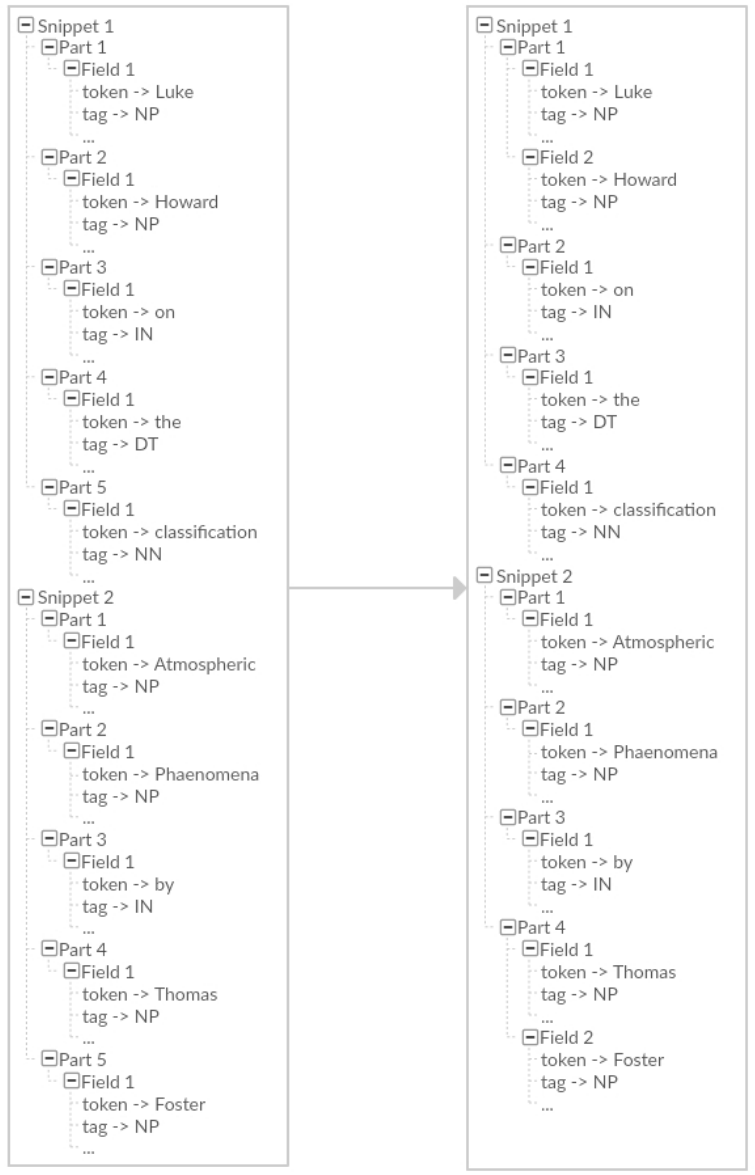
\includegraphics[scale=0.53]{obrazky-figures/SnippetsPartsFields.png}
	\caption{Struktura \emph{\uv{snippets-parts-fields}} před a po provedení sloučení polí}
    \label{SnippetsPartsFieldsLbl}
\end{figure}

\section{Diagram tříd serverové aplikace}
\renewcommand{\bottomfraction}{0.85}
\begin{figure}[ht]
\vspace*{-3cm}
	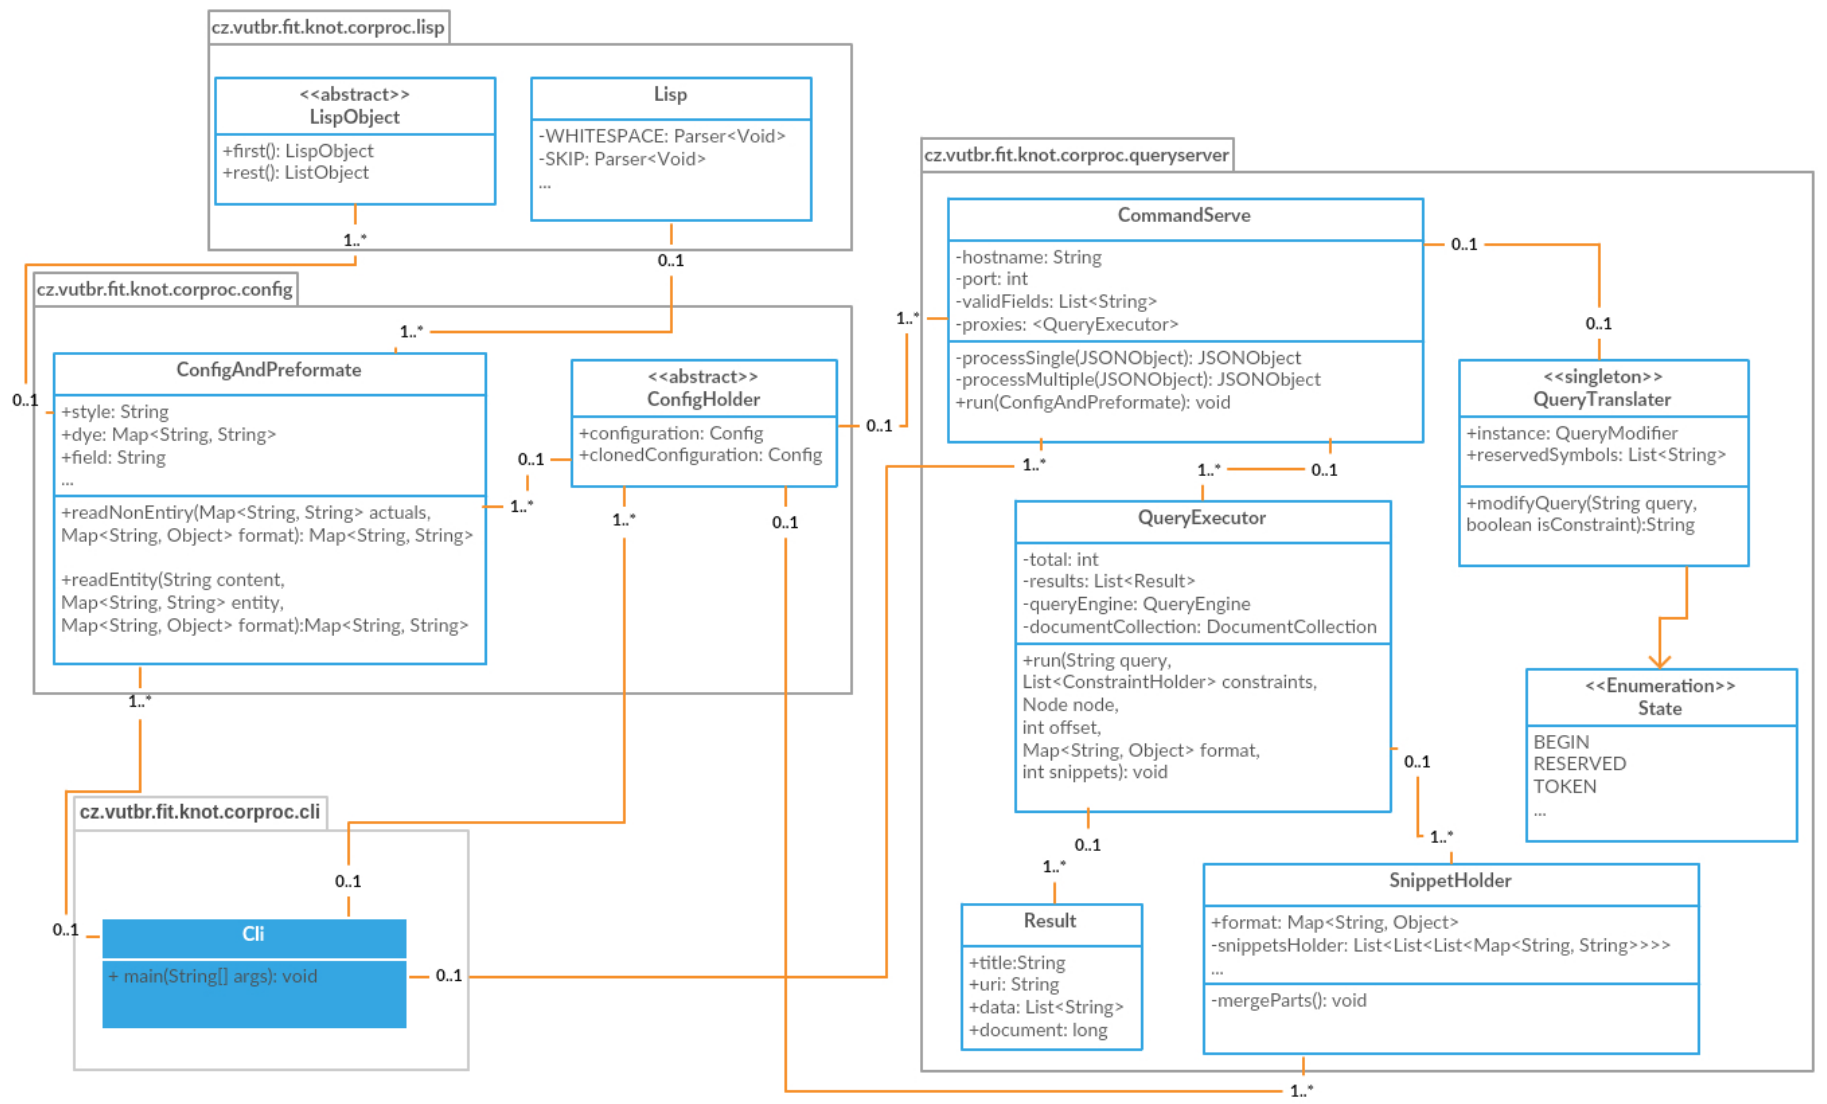
\includegraphics[scale=0.38, angle=90]{obrazky-figures/ClassDiagrameServer.png}
	\caption{Diagram tříd serverové části aplikace. Na diagramu jsou uvedené základní třídy s neúplným seznamem metod a atributů}
    \label{ClassDiagramServerLbl}
\end{figure}

\section{Diagram tříd klientské aplikace}
\begin{figure}[ht]
\vspace*{-3cm}
	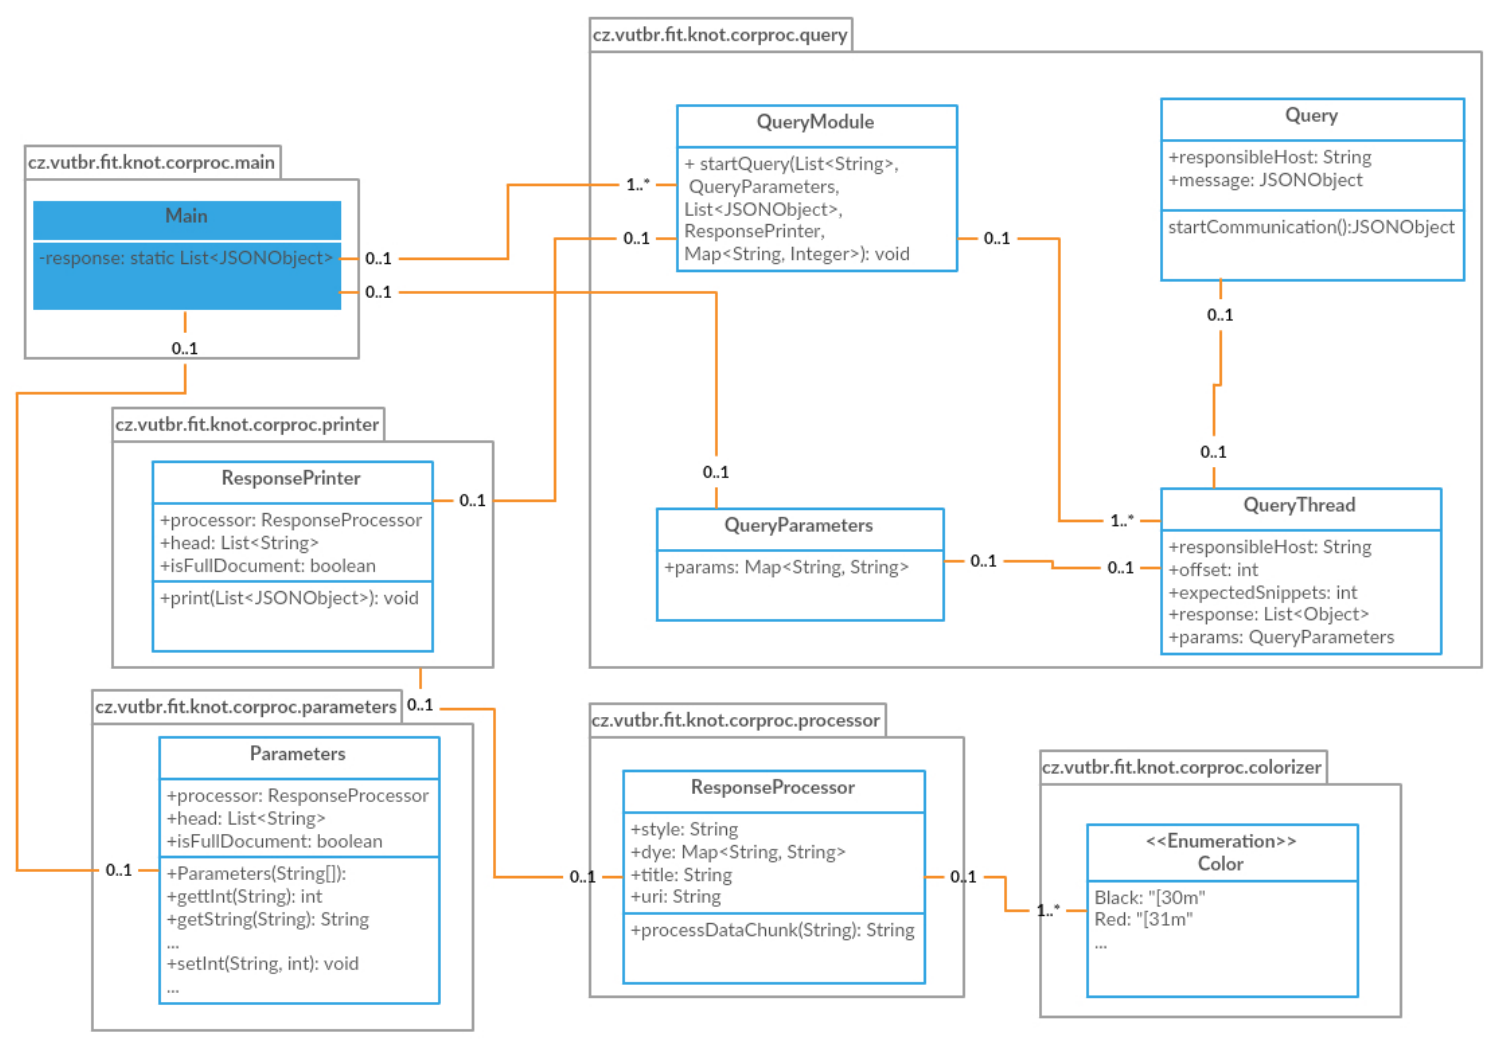
\includegraphics[scale=0.45, angle=90]{obrazky-figures/ClientClassDiagram.png}
	\caption{Diagram tříd klientské části aplikace. Na diagramu jsou uvedené základní třídy s~neúplným seznamem metod a atributů}
    \label{ClientClassDiagrameLbl}
\end{figure}

